\section{Preliminary}\label{sec:preliminary}
Large language models (LLMs), pretrained on vast corpora, have demonstrated superior capabilities in context understanding and logical reasoning. 
These models have achieved remarkable success across a wide range of tasks in various domains, including natural language processing~\cite{DBLP:journals/corr/abs-2307-06435, DBLP:journals/csur/MinRSVNSAHR24,xu2024large} 
and 
computer vision~\cite{DBLP:conf/nips/LiuLWL23a,DBLP:journals/pami/ZhangHJL24,DBLP:journals/corr/abs-2306-16410}.
Mainstream LLMs, such as GPT~\cite{bubeck2023sparks}, LLaMA~\cite{DBLP:journals/corr/abs-2302-13971}, and DeepSeek~\cite{DBLP:conf/acl/DaiDZXGCLZYWXLH24}, 
are primarily built on the transformer architecture~\cite{vaswani2017attention}. 
To explore the role of Key-Value (KV) cache management in accelerating LLM computations,
we first outline the core components of the transformer model and then introduce the mechanisms for managing the KV cache
to accelerate the LLMs.
Important notations in this survey are summarized in Tab.~\ref{tab:notation}.




\subsection{Transformer Architecture}\label{ssec:transformer}
Transformers~\cite{vaswani2017attention} have become the backbone of LLMs due to their ability to efficiently capture long-range dependencies sequential data, such as text.
This capability makes them particularly well-suited for tasks like machine translation, text generation, and image captioning.
The transformer architecture follows an encoder-decoder structure, where most LLMs utilize only the decoder component.
We first introduce the core components of the Transformer decoder and then describe the critical auto-regressive generation mechanism. 
Particularly, we do not describe certain components in transformer, such as normalization, as they do not impact the understanding of KV cache management.

\begin{table}[t]
    \centering
    \caption{Notation Summary}
    \label{tab:notation}
    \begin{tabular}{c|l}
        \toprule
        \textbf{Symbol} & \textbf{Definition} \\
        \midrule
        $X$ & Input sequence of tokens \\ \hline
        
        $\mathbf{X}$ & Dense representations of  $X$ \\ \hline

        $d_x$ & Dimensionality of the input embeddings. \\\hline

        
        $\mathbf{E}$ & Embedding matrix $\mathbf{E} \in \mathbb{R}^{d_{\text{vocab}} \times d_x}$. \\ \hline
        
        $PE(X)$ & Positional encoding \\ \hline
        
        $\mathbf{Q}_i, \mathbf{K}_i, \mathbf{V}_i$ & Query, Key, and Value matrices \\  \hline

         $d_k, d_v$ & Query/Key and Value dimension \\\hline

        $\mathbf{W}_{Q_i}, \mathbf{W}_{K_i}, \mathbf{W}_{V_i}$ & Weight matrices for computing $\mathbf{Q}_i, \mathbf{K}_i, \mathbf{V}_i$. \\\hline
        
        $\mathbf{Z}_i$ &  Self-attention Output  \\\hline
        
        $\mathbf{W}_O$ & Weight matrix \\\hline
        
        $\mathbf{W}_1, \mathbf{W}_2$ & Weight matrices \\ \hline
        
        $\mathbf{b}_1, \mathbf{b}_2$ & Bias vectors \\\hline
        
      %  $d_o$ & Dimensionality of the concatenated output of multiple attention heads. \\
       % $d_1, d_2$ & Dimensionality of intermediate and output layers in the Feed Forward Network (FFN). \\
       
        $t$ &  Sequence length index \\\hline
        
        $t_c$ & Number of tokens stored in the KV cache. \\ \hline
        
        $\mathbf{K}_i^t, \mathbf{V}_i^t$ & Key and Value at step $t$ \\ \hline        
        $\mathbf{\hat{K}}_i^{t-1}, \mathbf{\hat{V}}_i^{t-1}$ & Cached Key and Value \\\hline
        
        $h$ & Number of attention heads per layer \\\hline
        
        
        $L$ & Number of transformer layers \\\hline
        
      %  $\mathbf{h}_t$ & Hidden state of the LLM at decoding step $t$. \\
        
       % $\mathbf{W}_{\text{out}}, \mathbf{b}_{\text{out}}$ & Output projection matrix and bias vector for predicting the next token. \\
        
        $P(x_{t+1} | x_1, \cdots, x_t)$ & Conditional probability \\
       % $\text{Softmax}$ & Softmax function used to compute attention weights or output probabilities. \\
        \bottomrule
    \end{tabular}
\end{table}

\subsubsection{Transformer Decoder}\label{ssec:decoder}
As shown in Figure~\ref{fig:transformer}, a decoder-based transformer architecture is composed of multiple stacked Transformer blocks, each designed to process sequential data effectively. 
Typically, a Transformer block consists of two core components, i.e., a Multi-Head Self-Attention (MHSA) mechanism and a Feed Forward Network (FFN). 
These blocks are arranged sequentially, where the output of one block is passed as input to the next. This iterative design allows the model to refine its understanding of the input sequence progressively, making it highly effective for tasks such as text generation and language modeling.


\noindent \textbf{Positional Encoding.}
Before the input sequence is processed by the Transformer blocks, it undergoes a preprocessing phase. 
First, a tokenizer processes the input sentence $X$ by splitting it into discrete units, such as words or subwords. The resulting sequence can be represented as 
${X} = [x_1, x_2, \cdots, x_{|X|}]$.
These tokens are then mapped to dense vector representations using an embedding layer, i.e., $\mathbf{X} = \mathbf{I}_X  \mathbf{E}^{\top}$,
where $\mathbf{I}_{X} \in \{0,1\}^{n \times d_{\text{vocab}}}$ represents the one-hot vector of tokenized input $X$, $\mathbf{E} \in \mathbb{R}^{d_{\text{vocab}} \times d_x}$ is the embedding matrix, 
and $\mathbf{X}=[\mathbf{x}_1, \mathbf{x}_2, \cdots, \mathbf{x}_{|X|}]\in \mathbb{R}^{n \times d_{x}}$ is the resulting matrix of embedded token representations.
Since the Transformer architecture does not inherently account for the order of tokens in a sequence, \textbf{positional encodings} are added to the token embeddings $\mathbf{X}$ to incorporate positional information. This can be expressed as $\mathbf{X}=\mathbf{X}+ PE(X)$,
where $PE(X) \in \mathbb{R}^{n \times d_x}$ represents a function~\cite{zhao2023length,zheng2021rethinking,su2024roformer} (e.g., sine and cosine-based positional encoding) that generates positional embeddings for the input ${X}$.


\noindent \textbf{Transformer Block.}
Once the input features are prepared, they are passed through a series of stacked Transformer blocks. Each block begins with the Multi-Head Self-Attention (MHSA) mechanism, which captures both local and global dependencies. For each token, the self-attention mechanism computes a weighted sum over all other tokens in the sequence, where the weights are derived from the similarity between the tokens.
Particularly, since the operations within each transformer block are identical, we use a single transformer block as an example.
Specifically, given the input to a block, denoted as $\mathbf{X} \in \mathbb{R}^{|X| \times d}$, the MHSA mechanism computes the query vectors $\mathbf{Q}_i \in \mathbb{R}^{|X| \times d_k}$, key vectors $\mathbf{K}_i \in \mathbb{R}^{|X| \times d_k}$, and value vectors $\mathbf{V}_i \in \mathbb{R}^{|X| \times d_v}$. These vectors are obtained through learned linear transformations as follows:
\begin{align}\label{eq:qkv}
\mathbf{Q}_i = \mathbf{X}\mathbf{W}_{Q_i}, \quad
\mathbf{K}_i = \mathbf{X}\mathbf{W}_{K_i}, \quad
\mathbf{V}_i = \mathbf{X}\mathbf{W}_{V_i},
\end{align}
where $\mathbf{W}_{Q_i}\in \mathbb{R}^{d_x \times d_k}$, $\mathbf{W}_{K_i} \in \mathbb{R}^{d_x \times d_k}$
and $\mathbf{W}_{V_i} \in \mathbb{R}^{d_x \times d_v}$ are the learned weight parameters.
Then, the self-attention operation is applied to each triple $(\mathbf{Q}_i, \mathbf{K}_i, \mathbf{V}_i)$, and obtain  the output of the $i$-th attention head $\mathbf{Z}_i$ as follows:
\begin{equation}\label{eq:self_attention}
\mathbf{Z}_i = \text{Attention}(\mathbf{Q}_i, \mathbf{K}_i, \mathbf{V}_i) = \text{Softmax}\left(\frac{\mathbf{Q}_i \mathbf{K}_i^\top}{\sqrt{d_k}}\right) \mathbf{V}_i,
\end{equation}
where  $\sqrt{d_k}$  is a scaling factor to ensure the numerical stability. To capture diverse relationships, multiple attention with $h$ heads are applied to $\mathbf{X}$ in parallel, and their outputs are concatenated with one transformation as follows:
\begin{align}\label{eq:self_attention_concat}
\mathbf{Z}=\text{Concat}(\mathbf{Z}_1, \mathbf{Z}_2, \dots, \mathbf{Z}_h)\mathbf{W}_O,
\end{align}
where \text{Concat} is concatenation operation and $\mathbf{W}_O \in \mathbb{R}^{d_v \times d_o}$ is the trainable parameters.




Following the self-attention mechanism, 
the output is passed through a \textbf{Feed Forward Network (FFN)}. The FFN is a fully connected neural network that applies two linear transformations separated by a nonlinear activation function $\sigma(\cdot)$ (e.g, ReLU~\cite{agarap2018deep}) :
\begin{align}\label{eq:ffn}
    \text{FFN}(\mathbf{Z}) = \sigma(\mathbf{Z}\mathbf{W}_1 + \mathbf{b}_1)\mathbf{W}_2 + \mathbf{b}_2
\end{align}
where $\mathbf{W}_1 \in \mathbb{R}^{d_o \times d_1}$ and $\mathbf{W}_2 \in \mathbb{R}^{d_1 \times d_2}$ are  two  parameters.
Also, $\mathbf{b}_1 \in \mathbb{R}^{d_1}$ and $\mathbf{b}_2 \in \mathbb{R}^{d_2}$ are two bias vectors.

\subsubsection{Auto-regressive Generation Mechanism}\label{ssec:auto_regressive}
LLMs employ an autoregressive mechanism to generate text token by token, with each token conditioned on the previously generated ones. This iterative process ensures that the output sequence remains coherent and contextually appropriate.
Formally, given an input sequence of tokens $X = [x_1, x_2, \cdots, x_t]$, 
the model predicts the next token $x_{t+1}$ at each decoding step $t$ by modeling the conditional probability distribution as follows:
\begin{equation}
P(x_{t+1} | x_1, x_2, \cdots, x_t) = \text{Softmax}(\mathbf{h}_t \mathbf{W}_{\text{out}} + \mathbf{b}_{\text{out}}),
\end{equation}
where $\mathbf{h}_t \in \mathbb{R}^{d_h}$ represents the hidden state of the LLM regarding $X$ at step $t$, $\mathbf{W}_{\text{out}} \in \mathbb{R}^{d_h \times vocab}$ is the output projection matrix, and $\mathbf{b}_{\text{out}}$ is the bias vector. 
The softmax function converts the logits into a probability distribution over the vocabulary.
Then,
at each decoding step, the model generates the next token $x_{t+1}$ by sampling from the predicted probability distribution:
\begin{equation}
x_{t+1} \sim P(x_{t+1} | x_1, x_2, \cdots, x_t).
\end{equation}
The generated token $x_{t+1}$ is then appended to the sequence $X=[x_1,\cdots,x_t,x_{t+1}]$, and the process continues until a special end-of-sequence (EOS) token is generated or a predefined maximum length is reached.



 \begin{figure}[t]
    \centering
    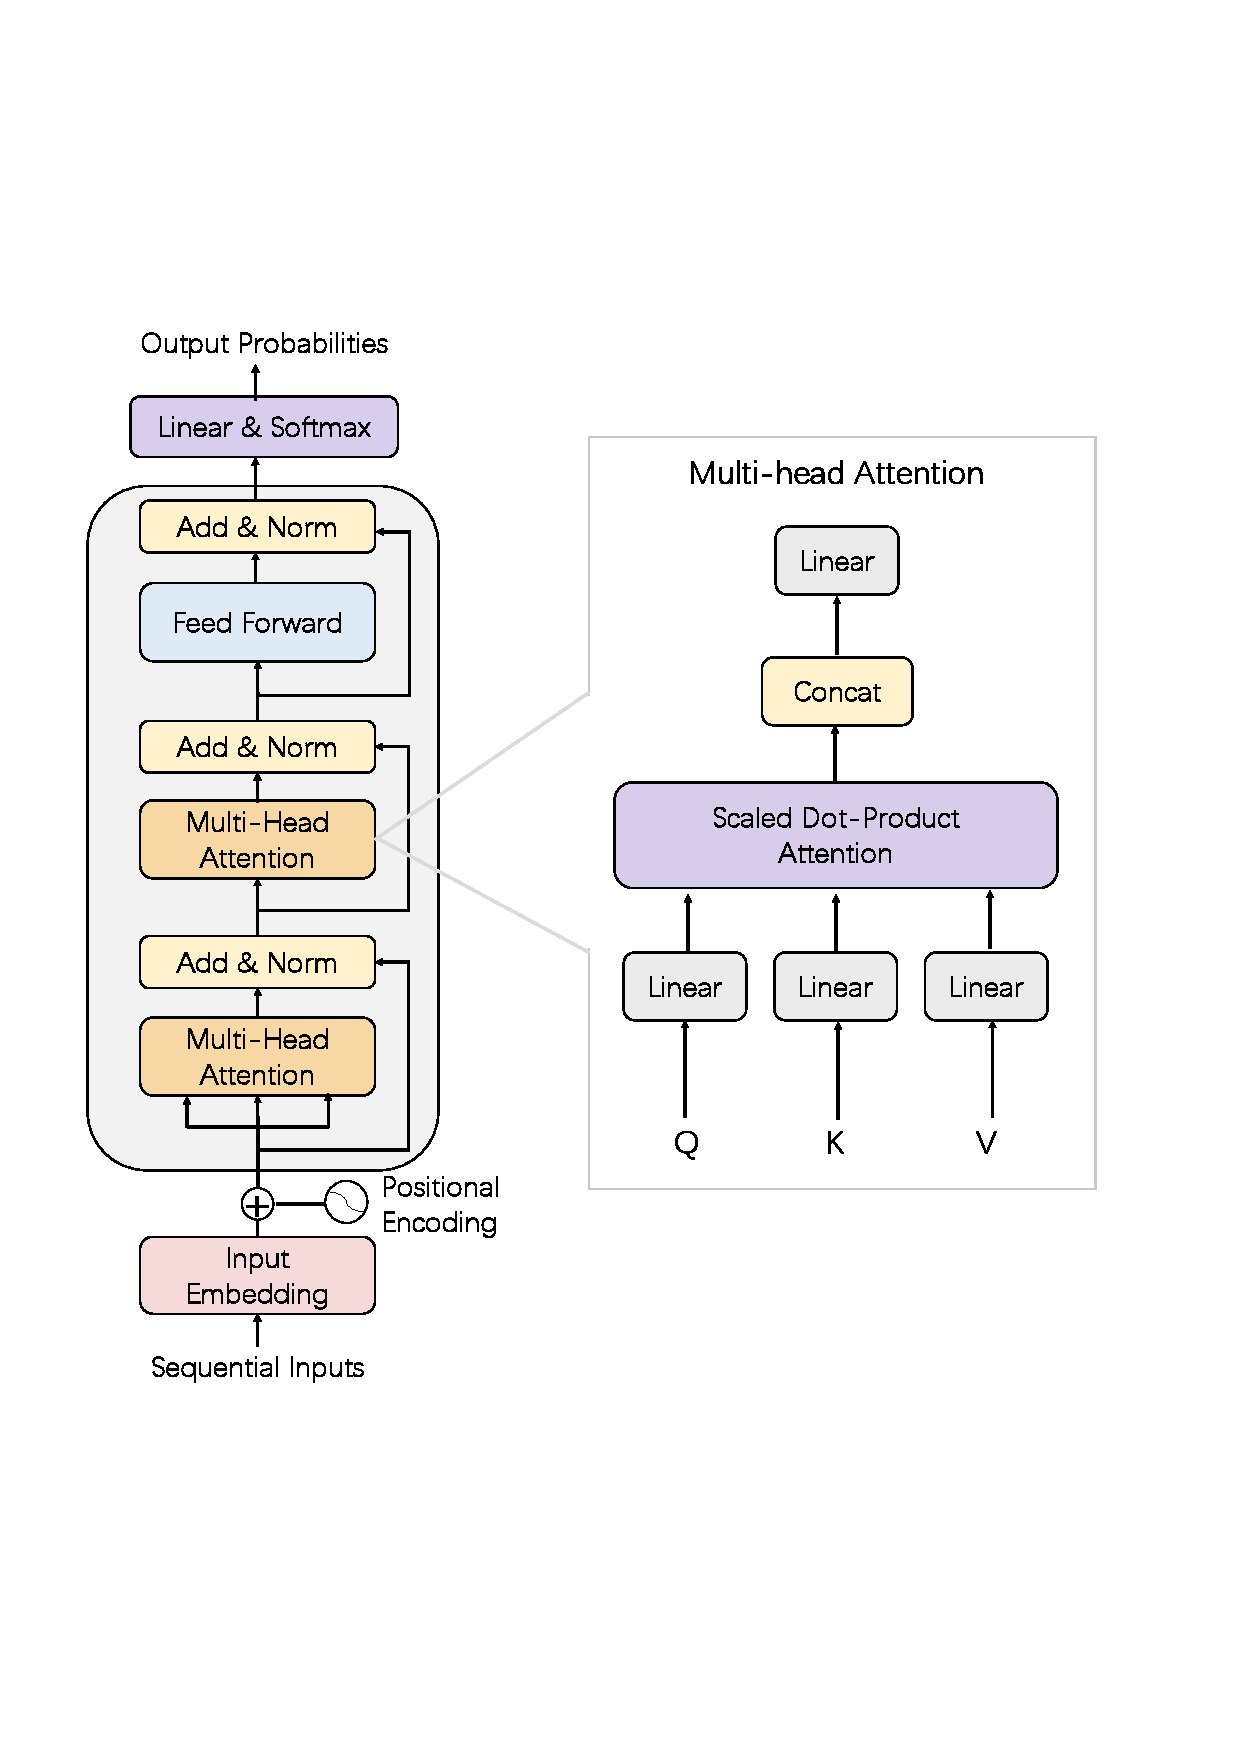
\includegraphics[width=0.88\linewidth]{figures/transfomer.pdf}
    \caption{The decoder-only Transformer for LLMs.}
    \label{fig:transformer}
\end{figure}


 


 

\subsection{Key-Value Cache in Transformer Models}\label{ssec:kv_cache}
Auto-regressive generation is a powerful mechanism that enables LLMs to produce high-quality, contextually coherent text. 
However, it presents computational challenges for long sequences, as the Keys and Values need to be recomputed for each token during the generation process. The KV cache optimization addresses this issue by storing the previously computed Keys and Values and reusing them for subsequent token generation, thereby reducing redundant computations and improving inference efficiency.


\subsubsection{Auto-regressive Generation with KV Cache}
Here, we describe how caching KV pairs of tokens accelerates LLM inference. Specifically, at each decoding step \( t \), the model performs self-attention over the entire sequence \( X = [x_1, \cdots, x_{t-1}, x_t] \) to generate the next token \( x_{t+1} \). This process requires the computation of Keys and Values matrices for all previously processed tokens in \( X = [x_1, \cdots, x_t] \).
Notably, when generating the token \( x_t \), the LLM has already computed the Keys and Values for the tokens in \( X[1:t-1] = [x_1, \cdots, x_{t-1}] \). The KV cache optimizes this process by storing the previously computed Keys and Values  matrices for \( X[1:t-1] \) and reusing them, thereby only requiring the computation of Keys and Values for the new token \( x_t \). This significantly improves efficiency by eliminating redundant computations.

Formally, at decoding step $t$, the new token embedding $\mathbf{x}_t$ is used to compute the query vector $\mathbf{q}^t_i$, key vector $\mathbf{k}^t_i$, and value vector $\mathbf{v}^t_i$ as follows:
\begin{align}
\mathbf{q}_i^t &= \mathbf{x}_t \mathbf{W}_{Q_i}, \quad
\mathbf{k}_i^t  = \mathbf{x}_t \mathbf{W}_{K_i}, \quad
\mathbf{v}_i^t  = \mathbf{x}_t \mathbf{W}_{V_i},
\end{align}
The newly computed $\mathbf{k}_i^t $ and $\mathbf{v}_i^t $ are then appended to the cached key and value matrices from previous steps:
\begin{align}
\mathbf{K}_i^{t} &= \text{Concat}(\mathbf{\hat{K}}_i^{t-1}, \mathbf{k}_i^t ), \ 
\mathbf{V}_i^{t} = \text{Concat}(\mathbf{\hat{V}}^{t-1}_i, \mathbf{V}_i^t ),
\end{align}
where $\mathbf{\hat{K}}_i^{t-1} \in \mathbb{R}^{t-1 \times d_k}$ and $\mathbf{\hat{V}}_i^{t-1} \in \mathbb{R}^{t-1 \times d_v}$ represent the cached key and value matrices of tokens in $X[1:t-1]$. 
These cached matrices are then used in the scaled dot-product attention computation for token $x_t$.
%which avoids re-computing attention for previously processed tokens. 
The attention output $\mathbf{z}^t_i$ for the token $x_t$ at step $t$ is calculated as:
\begin{align}
\mathbf{z}^t_i = \text{Softmax}\left(\frac{\mathbf{q}_i^t {\mathbf{K}_i^t}^\top}{\sqrt{d_k}}\right) \mathbf{V}_i^t,
\end{align}
\noindent Then, a similar KV reuse process can be applied to different attention heads in each layer of the LLM.


 
 

\subsubsection{Time and Space Complexity Analysis}\label{sssec:time_space}
Given a transformer-based $L$-layer LLM with $h$ attention heads per layer and an input sequence of length $X = [x_1, \cdots, x_t]$, we analyze the time saved and the space required to store cached KV pairs. For simplicity, we assume the Keys and Values of $t_c$ tokens are stored for all heads across all LLM layers.

\noindent \underline{\textbf{Saved Time.}} 
    For each token,
    the saved computation time comes from avoiding the repeated computation of Keys and Values in Equation~\eqref{eq:qkv}, self-attention result in Equation~\eqref{eq:self_attention}, 
    and linear transformation  in  Equation~\eqref{eq:self_attention_concat}.
     We omit the time analyze on operations in transformer that do not affect  the understanding of KV cache acceleration, such as layer norm and position encoding.

    %and non-linear transformation  in  Equation~\eqref{eq:self_attention_concat} and~\eqref{eq:ffn}.
\begin{itemize}[leftmargin=10pt]
    \item \textbf{QKV Computation.} 
    The time of computing Queries, Keys and Values for each token in Equation~\eqref{eq:qkv} is $\triangle_1 = O(2d_xd_k + d_xd_v)$.
  
    \item  \textbf{Self-attention Result.} 
    Additionally, computing each attention result $\mathbf{z}_i$ in Equation~\eqref{eq:self_attention} takes $O(t(d_k + d_v))$.
    %where $t$ is the sequence length. 

   \item \textbf{Linear Transformation.}
    To merge the $h$ attention results in  Equation~\eqref{eq:self_attention_concat} 
    %and compute the forward result in Equation~\eqref{eq:ffn}, 
    the time is $\triangle_2 = O(hd_v+d_vd_o)$. 

\end{itemize}
Therefore, for $t_c$ cached tokens across $h$ attention heads and $L$ layers, the total saved computation time is:
\begin{align}
    %O\left(L\cdot h \cdot t_c \cdot t \cdot (d_k+d_v)+ L\cdot h \cdot t_c\cdot \triangle_1 \right)
    O\left(L\cdot h \cdot t_c \cdot t \cdot (d_k+d_v)+ L\cdot h \cdot t_c\left(\triangle_1 + \triangle_2\right)\right)
\end{align}
\noindent Thus, the saved time is directly proportional to the number of cached tokens $t_c$, 
significantly accelerating model computation, especially for longer sequences (when $t$ is large).



\noindent \underline{\textbf{Extra Space.}}
Compared to computation without caching, additional space is required to store the cached KV pairs for $t_c$ tokens across $h$ attention heads and $L$ layers. Assuming each Key and Value is stored in Float16 precision, the total extra space needed can be expressed as:
\begin{align}
    O(L\cdot h \cdot t_c \cdot 2 \cdot sizeof(Float16))    
\end{align}
\noindent 
Thus, for the same LLM model, the extra space required to store the KV pairs primarily depends on the number of cached tokens and the precision of the cached Keys and Values. 
To address this, existing approaches explore various techniques to reduce the extra space consumption, such as caching only the most important Keys and Values or applying quantization techniques to lower the bit precision of the stored Keys and Values.






 


\subsection{Challenges in KV Cache Management}\label{ssec:kv_cache_challenge}
As analyzed in Sec.~\ref{sssec:time_space}, 
reusing cached KV pairs enables the LLM to avoid recomputing past tokens, resulting in significant speedups during inference. However, as sequence lengths grow, the size of the KV cache increases proportionally, placing significant pressure on memory. Consequently, it becomes challenging to manage this cache effectively to accelerate LLM computation without excessive space usage.

\begin{itemize}[leftmargin=10pt]
    \item \textbf{Cache Eviction Policies:} 
    Determining which items to evict when the cache reaches its capacity is a complex problem. Popular policies~\cite{podlipnig2003survey} like Least Recently Used (LRU) or Least Frequently Used (LFU) do not align with LLMs  patterns, leading to suboptimal performance.

    \item \textbf{Memory Management:} 
    The memory required for the KV cache grows linearly with both the sequence length and the number of layers, which can quickly exceed the hardware memory limits, especially for long sequences. Consequently, managing the collaboration between different types of storage hardware (e.g., GPU, CPU, or external memory) becomes a significant challenge.




    
    \item \textbf{Latency Bottlenecks:} Accessing and updating the cache at each decoding step can introduce latency, particularly for hardware with limited memory bandwidth.

    \item \textbf{Compression Trade-offs:} Compressing the KV cache can reduce memory usage but may degrade model performance if key information is lost.

    \item \textbf{Dynamic Workloads:} Handling dynamic and unpredictable workloads, where access patterns and data requirements frequently change, requires adaptive caching strategies that can respond in real time.


    \item \textbf{Distributed Coordination:} In distributed KV caches, maintaining coordination across multiple nodes to ensure consistency, fault tolerance, and efficient resource usage adds significant complexity.

\end{itemize}